\documentclass{seminarreport}
\usepackage{seminarreportcommands}

\defstudentname{John Doe}
\defstudentregno{1200XXXXX}
\defhisher{his}
\defsemester{seventh}
\defstudyyear{2019~-~2020}		% ~ is for non breaking space
\defguide{John Doe II}

\title{The Title of the work you are doing goes here}

\begin{document}
	\pagenumbering{roman}
	\makeseminarfirstpage
	\makeseminarsecondpage
	\bonafide
	\acknowledgement{\lipsum[1]}
	\newpage
	\fakesection{Table of contents}
	\tableofcontents
	\newpage
	\fakesection{Tables Index}
	\newpage
	\listoftables			% Comment if you have no tables in your doc
	\fakesection{Figures Index}
	\listoffigures
	\newpage
	\pagenumbering{arabic}
	\section{Abstract}
	\setcounter{page}{1}
	\lipsum[2]
	\section{Introduction}
	\lipsum[3]
	\section{Literature Review}
	\subsection{Paper 1}
		\lipsum[4]
	\subsection{Paper 2}
		\lipsum[5]
	\section{Current Solution}
		\lipsum[6]
	\section{Proposed Solution}
		\lipsum[7]
	\section{Results}
		\lipsum[8]
	\begin{table}[h!]
		\centering
		\begin{tabular}{||c c c c||} 
			\hline
			Col1 & Col2 & Col2 & Col3 \\ [0.5ex] 
			\hline\hline
			1 & 6 & 87837 & 787 \\ 
			2 & 7 & 78 & 5415 \\
			3 & 545 & 778 & 7507 \\
			4 & 545 & 18744 & 7560 \\
			5 & 88 & 788 & 6344 \\ [1ex] 
			\hline
		\end{tabular}
		\caption{Dummy Table}
		\label{table:1}
	\end{table}
	\begin{figure}[h]
		\caption{Spiral image}
		\centering
		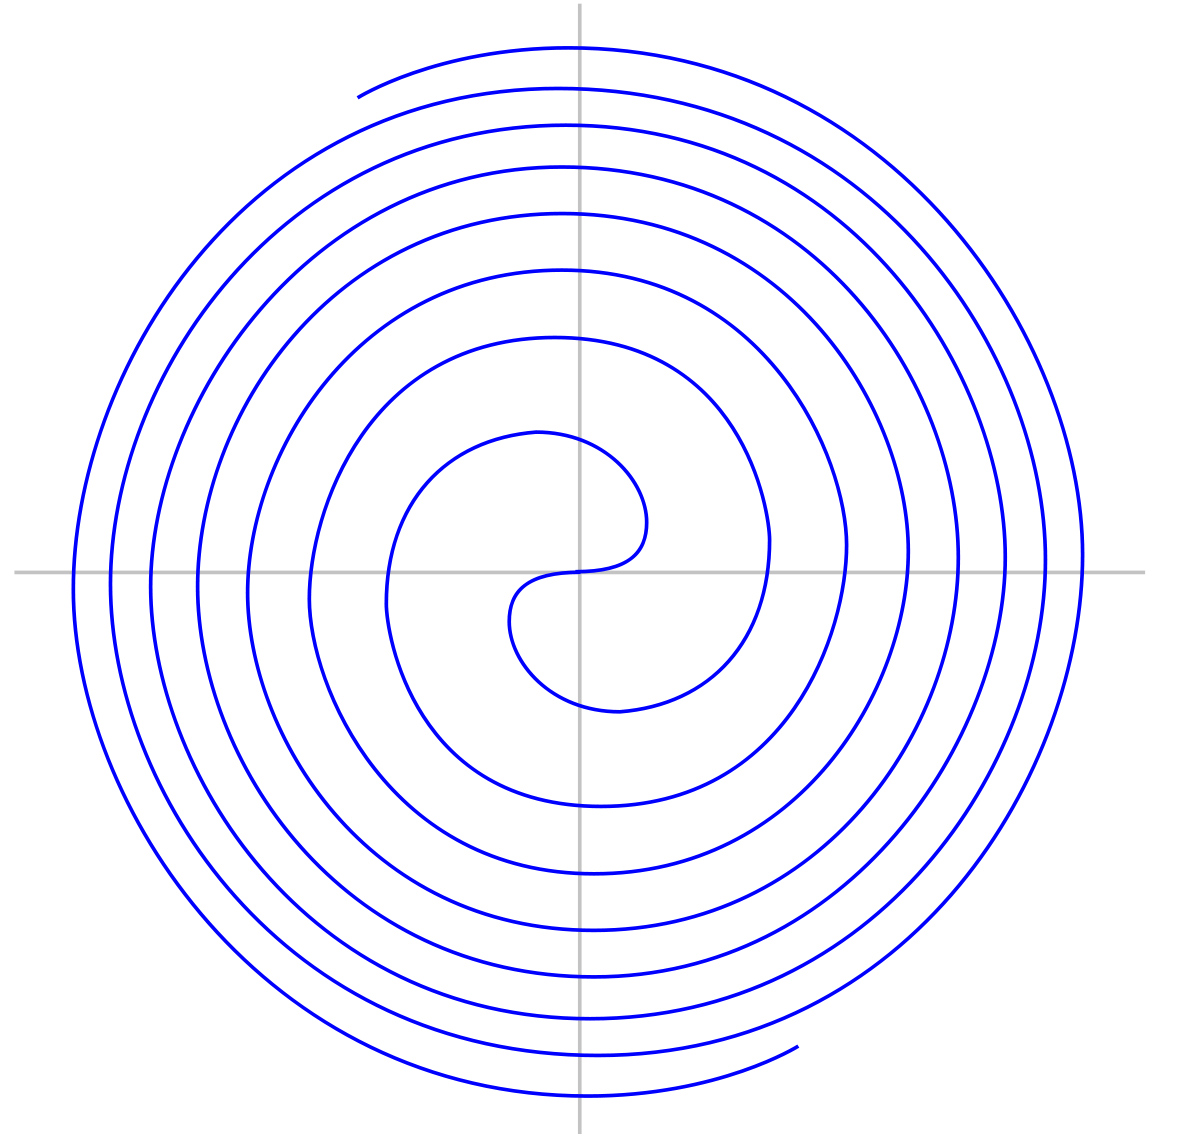
\includegraphics[width=0.5\textwidth]{images/spiral}
	\end{figure}

	\section{Conclusion}
	This is just some sample textI'm adding to show how citations\cite{einstein} work. This \cite{latexcompanion} is another example.
	\newpage
	\bibliography{sample} 
	\bibliographystyle{ieeetr}
\end{document}